\documentclass[fleqn]{article}
\usepackage{fullpage}
\usepackage{amsmath}
\usepackage{enumitem}
\usepackage{amssymb}
\usepackage{listings}
\usepackage{hyperref}
\usepackage{tikz}
\usepackage{algpseudocode}
\usepackage{algorithm}
\usepackage{multicol}

\renewcommand{\vec}[1]{\mathbf{#1}}

\DeclareMathOperator*{\argmax}{arg\,max}
\usetikzlibrary{arrows}
\lstset{basicstyle=\ttfamily, mathescape}
\graphicspath{{./img/}}

\usepackage[utf8]{inputenc}

% Default fixed font does not support bold face
\DeclareFixedFont{\ttb}{T1}{txtt}{bx}{n}{12} % for bold
\DeclareFixedFont{\ttm}{T1}{txtt}{m}{n}{12}  % for normal

% Custom colors
\usepackage{color}
\definecolor{deepblue}{rgb}{0,0,0.5}
\definecolor{deepred}{rgb}{0.6,0,0}
\definecolor{deepgreen}{rgb}{0,0.5,0}

\usepackage{listings}

% Python style for highlighting
\newcommand\pythonstyle{\lstset{
language=Python,
basicstyle=\tt,
otherkeywords={self},             % Add keywords here
keywordstyle=\tt\color{deepblue},
emph={MyClass,__init__},          % Custom highlighting
emphstyle=\tt\color{deepred},    % Custom highlighting style
stringstyle=\color{deepgreen},
frame=tb,                         % Any extra options here
showstringspaces=false            %
}}


% Python environment
\lstnewenvironment{python}[1][]
{
\pythonstyle
\lstset{#1}
}
{}

% Python for external files
\newcommand\pythonexternal[2][]{{
\pythonstyle
\lstinputlisting[#1]{#2}}}

% Python for inline
\newcommand\pythoninline[1]{{\pythonstyle\lstinline!#1!}}

\title{\textbf{Edibility of Mushroom Species}}
\author{
    \begin{tabular}{cccc}
            Ishaan Saxena      & Nikita Rajaneesh    & Swaraj Bhaduri     & Utkarsh Jain       \\
            isaxena@purdue.edu & nrajanee@purdue.edu & sbhadur@purdue.edu & jain192@purdue.edu
    \end{tabular}
}

% Document
\begin{document}
    \maketitle

    % 1
    \section{Introduction to the Problem}

    % 1.1
    \subsection{Definition of the Problem}

    Given a dataset $ \mathcal{D} $ with $ n=8124 $ samples where each sample represents a
    mushroom with features being the observations about the characterestics of the mushrooms
    such as odor, color, etc., we aim to test and compare various supervised learning models
    for the problem of classifying each sample into either poisonous or edible. Further,
    we will optimize the Hyperparameters of the model which initially performs the best
    on the dataset.\footnote{This dataset can be found at
    \href{https://www.kaggle.com/uciml/mushroom-classification}
    {https://www.kaggle.com/uciml/mushroom-classification}.}

    % 1.2
    \subsection{Data Description}

    We are given $ \mathcal{D} $ with $ n=8124 $ samples wherein each sample has the
    following 22 features (excluding the class label).

    \begin{multicols}{3}
        \begin{enumerate}
            \item cap-shape
            \item cap-surface
            \item cap-color
            \item bruises
            \item odor
            \item gill-attachment
            \item gill-color
            \item stalk-root
            \item stalk-surface-above-ring
            \item stalk-surface-below-ring
            \item stalk-color-above-ring
            \item stalk-color-below-ring
            \item veil-type
            \item veil-color
            \item ring-type
            \item spore-print-color
            \item habitat
            \item gill-spacing
            \item gill-size
            \item stalk-shape
            \item ring-number
            \item population
        \end{enumerate}
    \end{multicols}
    \noindent
    These features have been further enumerated in Appendix A.\\

    The labels are binary, namely edible (e) and poisonous(p). Within the original dataset,
    there are the following number of edible and poisonous mushrooms.

    \begin{python}
    >>> df['class'].value_counts()
    e    4208
    p    3916
    \end{python}

    % 1.3
    \subsection{Encoding the Data}

    Note that all the features in our dataset are categorical variables. As a result, to
    proceed with evaluation of model performance, we must first encode these variables
    into numerical/binary values.\\

    We need to deal with two kinds of categorical variables when encoding the features
    into numerical data. These are ordinal categorical variables and nominal categorical
    variables.\footnote{Information on which features are which kind of categorical
    variables can be found in Appendix A.} We will use different techniques to encode
    both of these kinds of categorical variables as they inherently represent different
    kinds of categorical data.

    \subsubsection{Nominal Categorical Variables}

    To encode nominal categorical variables, we will use one-hot binary features. For
    instance, if a feature $ f $ from a feature set $ \mathcal{F} $ has $ k $ different
    categorical values, we can create $ k $ different binary features for each feature
    $ f $ of this kind. This is done because the values of each such feature do not hold
    any ordinal information, in that there should not be different weights for having a
    specific value of a specific feature.

    \subsubsection{Ordinal Categorical Variables}

    The ordinal categorical variables, on the other hand, have been encoded as numerical
    labels, as these informations contain valueable information about the 'scale' of a
    certain feature. For instance, if a feature $ f $ from a feature set $ \mathcal{F} $
    has $ k $ different features, it would be changed into numeric values
    $ i \in 0,1,...,k-1$.

    \subsubsection{Encoding Process}

    The following code segment is used to encode the data.\footnote{This can be found in
    the data.py file.}

    \begin{python}
def encode(df):
    # Encode Ordinal Variables
    ordinal_columns = ['gill-spacing', 'gill-size',
            'stalk-shape', 'ring-number', 'population', 'class']
    columns = ordinal_columns[:]

    for column in columns:
        df[column] = df[column].astype('category')

        columns = df.select_dtypes(['category']).columns
        df[columns] = df[columns].apply(lambda x: x.cat.codes)

    # Encoding Nominal Variables
    columns = ordinal_columns[:]

    for column in df:
        if column not in columns:
            dummies = pd.get_dummies(df.pop(column))
            column_names = [column + "_" + x for x in dummies.columns]
            dummies.columns = column_names
            df = df.join(dummies)

    return df
    \end{python}

    \noindent
    We can now see how our encoded dataset $ \mathcal{D} $ is shaped, and then proceed
    further in our task to classify data.

    \begin{python}
>>> X, y = data.load() # data.load() calls data.encode()
>>> X.shape
(8124, 107)
>>> y.shape
(8124,)
    \end{python}

    % 2
    \section{Machine Learning Pipeline}
    Before we proceed, let's briefly go through our machine learning pipeline. Consider
    the encoded dataset $ \mathcal{D} $. Given this dataset, we will proceed to solve our
    classification problem by taking the following steps:

    \begin{enumerate}
        \item Feature selection and test-train split:\footnote{See get\_reduced\_data in data.py}
        \begin{enumerate}[label=\roman*.]
            \item Split $ \mathcal{D} $ into the training/validation set $ D $ and testing
            set $ D' $.
            \item Get a set of $ f $ best features from $ D $; call this set $ \mathcal{F} $.
            \item Create new training $ Z $ and testing sets $ Z'_1, Z'_2 $ by
            choosing only the subset of features $ \mathcal{F} $ from $ D $ and $D'$ respectively.
        \end{enumerate}
        \item Model selection and hyperparameter tuning:\footnote{See modelSelection.py}
        \begin{enumerate}[label=\roman*.]
            \item Choose a set of models $ \mathcal{M} $ and a possible set parameters
            $ \mathcal{P} $ for each model.
            \item For each model $ M \in \mathcal{M} $, choose the best set of parameters
            $ P^* \in\mathcal{P} $ via hyperparameter tuning. Note that the hyperparameter
            tuning process trains a model on $ Z $ with each possible parameter and evaluates
            performance on $ Z'_1 $.
            \item Use $k$-fold Cross Validation on testing set $ Z'_2 $ to get mean accuracy
            and standard deviations for each model $ M \in \mathcal{M} $ with it's
            optimal hyperparameters $ P^* \in\mathcal{P} $.
            \item Compare models with hypothesis testing and choose best model.
        \end{enumerate}
    \end{enumerate}

    We will present the metrics and evaluation results for the best selected model.

    % 3
    \section{Feature Selection}

    % 3.1
    \subsection{The Need for Feature Selection}
    Feature selection is a useful technique when we want to better understand the input
    feature set. Having fewer features also leads to a more interpretable model, and is
    definitely helpful in our case, since we have just created over 100 features from
    which we want to derive a model to solve the classification problem. As a result,
    feature selection techniques can help us get a better idea of which features matter
    more or less while classifying our model.\\

    It is also important to note that feature selection helps us have a control over the
    complexity of the model. This is a very important aspect, as a less complex model
    is more useful for generalization.

    % 3.2
    \subsection{Feature Selection Technique}
    We are using Greedy Subset Selection for Feature Selection. Greedy Subset Selection is
    a greedy algorithm for selecting a good subset of feature coordinates. Greedy selection
    chooses optimum features by minimizing the mean squared error. After selecting a subset
    of features, it tries to add features based on whichever feature works best with the
    current subset.

        $$ S = S \cup \left[\text{argmin}_{j\notin S} \text{min}_{\theta_{S\cup j}}\left(\frac{1}{2}
        \sum_{t=1}^n (y_t-\theta_{S\cup j}\cdot\phi_{S\cup j}(x_t))^2\right)\right] $$

    \noindent
    GSS is computationally faster than Subset Selection. It is also more optimal
    in comparison to Foward-Fitting and Myopic Forward Fitting algorithms.

    % 3.3
    \subsection{Greedy Subset Selection Results}
    The following are the 46 best features and their weights obtained from Greedy Subset
    Selection:
    \begin{center}
        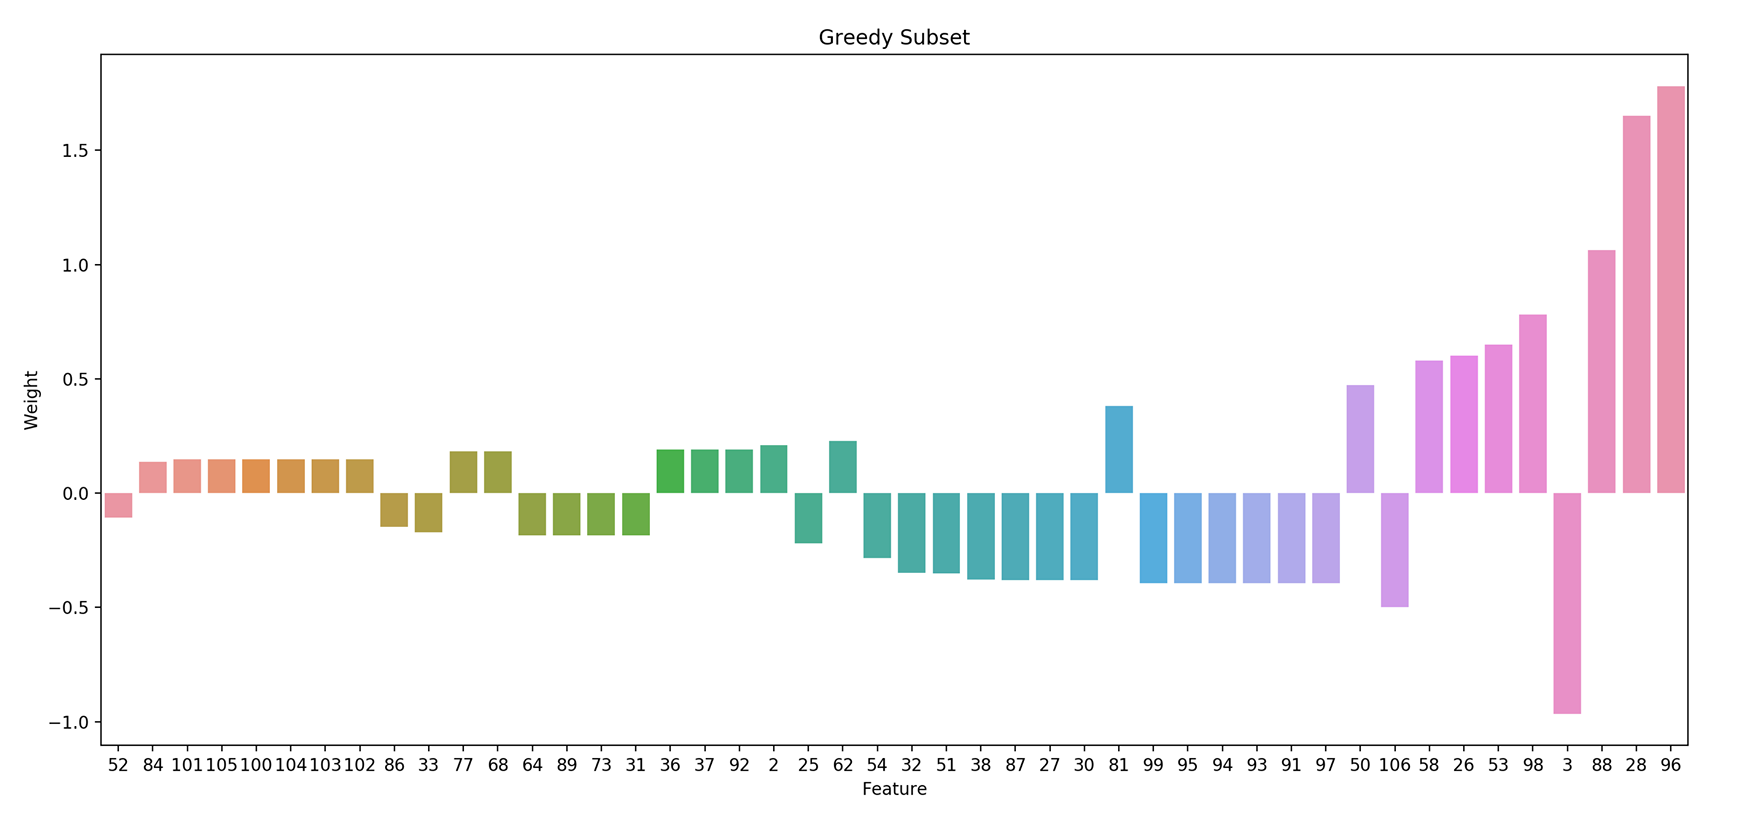
\includegraphics[scale=0.5]{46.png}
        \begin{figure}[!h]
            \caption{Greedy Subset Selection - 46 features with highest weights. Obtained from featureSelectionPlot.py}
        \end{figure}
    \end{center}

    Our processed data-set contains 8124 samples and 107 features. Hence, the need for
    reduction of features arises from the size of the dataset, specifically, the large
    number of features our models need to learn from and the fact that certain features
    have a high correlations making addition of all features redundant. Further, a lot of
    the features have little or no correlation with the class label and
    adding such features just plainly increases our computation time without actually
    helping our model make ‘better’ decisions (in some cases, they even increase noise and
    make the model's decisions worse).\\

    Thus, reduction of features increases the efficiency
    of training our models, helps us remove redundant features from our data set and
    learn only from features which have a considerable impact on our class labels.
    Reduction of features also helps in a control over complexity of some models, as it
    helps with better generalizability.\\

    The best feature, as can be seen in the graph above is Feature 96, namely,
    bruises-f. This is a boolean encoded feature, which is 1 if the mushroom does not have
    any bruises, and 0 if the mushroom has bruises. Now, let's have a look at the following
    code to understand why this is:
    \begin{python}
    >>> import data
    >>> X, _, y, _ = data.get_reduced_data(0.6, 1)
    >>> n = X.values.size
    >>>  np.sum((X.values.resize(n, ) == y))
    0
    \end{python}
    This indicates that in the training set $ Z = (X, y) $, on which feature selection has
    been performed, every mushroom with bruises is a poisonous mushroom (since a sum of
    zero indicates that for each instance of $ X $, the class label $ y\in\{0, 1\} $ was
    not equal to the value of $ X\in\{0, 1\} $). As such, this feature seems to be a very
    good identifier of the edibility of mushrooms.

    % 4
    \section{Cross Validation}
    We use cross-validation to evaluate the chosen predictive model by paritioning it into
    smaller train and test datasets wherein we train the model on the training set and
    evaluate it on the testing set. By using better cross-validation techniques, we can
    get a better understanding of how well our model will generalize, and whether we might
    be over or underfitting.\\

    In order to conduct cross validation for (i) tuning of hyperparameters
    \footnote{See Section 5} and (ii) evaluation of model performance \footnote{See Section 6},
    we use a form of nested cross validation as explained previously in our pipeline. We
    use a combination of $k$-Fold CV and Train-Validate-Test to make sure that any of the
    data used in either of the two evaluation sets has not been exposed to the models
    which are being tuned and evaluated before.

    \subsection{Basic Methodology}
    Given the original encoded dataset $ \mathcal{D} $, we create a 40:20:40 split,
    namely $ D, D'_1, D'_2 $. We conduct our feature selection process as descibed in the
    previous section on $ D $ to obtain a reduced subset of features $ \mathcal{F} $.
    This reduced subset of features is used to obtain $ Z, Z'_1, Z'_2 $, which are used
    as a train-validate-test sets respectively. Each model is initially trained with
    different hyperparameters on $ Z $, and evaluated on $ Z'_1 $ to get the best set of
    hyperparameters. Further, we conduct $k$-Fold CV on $ Z'_2 $ by used the optimal set of
    hyperparameters which we get from the previous step to evaluate the performance of a
    selected model on unseen data.

    \begin{center}
        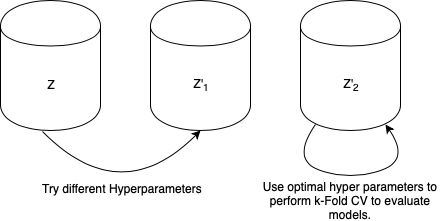
\includegraphics[scale=0.4]{tvt.png}
        \begin{figure}[!h]
            \caption{Cross Validation Model}
        \end{figure}
    \end{center}

    \subsection{Train-Validate-Test}
    We obtain the $ Z, Z' $ 40:60 split in the data.py file when creating a dataset
    with a reduced number of features. After doing so, we further split $ Z' $ into
    $ Z'_1, Z'_2 $ such that $ |Z| \approx 3200, |Z'_1| \approx 1600, |Z'_2| \approx 3200 $.
    Note that \underline{all splits are random}, and as a result, differing
    results may be obtain for different splits of the data.\footnote{As we'll see however,
    even with different splits, we get multiple models which consistently performs with
    over 98\% accuracy on the 5-Fold CV on $ Z'_2 $. We will use vc-Dimensions of these
    models along with results from hypothesis testing (Section 7) to compare these models
    further.}

    \subsection{$k$-Fold CV}

    Here, we are using $k$-Fold Cross Validation on 2, 5, and 10 folds. While we conduct
    $k$-Fold Cross Validation in all of these fold sizes, we will only compare models based on
    their performances in 5-folds.\\

    In $k$-Fold CV, we
    split the dataset into $k$ different folds. For each $i^{th}$ fold, where
    $ i = 1, 2,...,k $, we train on the remaining $ k-1 $ folds and evaluate on the single
    remaining fold. As a result, we get $ k $ different measures of the metrics which we
    are using for each model we evaluate using the cross-validation technique. These can
    be aggregated into a single metric as follows:

    $$  \hat\mu = \frac{1}{k} \sum_{1\leq i \leq k} M_i \text{, and }
        \hat\sigma^2 = \frac{1}{k} \sum_{1\leq i \leq k} (M_i - \hat\mu)^2 $$

    \noindent
    where $ M_i $ is the measure for the $i^{th}$ fold (here, it is accuracy). This
    aggregation may be used in a statistical hypothesis test to compare the performances
    of two different models.\\

    \noindent
    The following is our implementation of $k$-fold cross validation:\footnote{This can be
    found in the kfoldcv.py file.}

    \begin{python}
    # For each fold
    for i in range(k):
        # Find sets S and T
        lower = np.floor(float(n) * i / k).astype('int64')
        upper = np.floor(float(n) * (i + 1) / k - 1).astype('int64')
        T = range(lower, upper + 1)
        S = list(range(0, lower)) + list(range(upper + 1, n))

        # Get training data
        X_train = X[S, :]
        y_train = y[S]

        # Fit model
        m = model(**kwargs)
        m.fit(X_train, y_train)

        # Check prediction accuracy
        y_pred = m.predict(X[T])

        # Update Z values based on accuracy score
        Z[i] = metrics.accuracy_score(y[T], y_pred)

    # Return k-Fold results
    return Z
    \end{python}

    \noindent

    % 5
    \section{Hyperparameter Tuning}
    Before we conduct any evaluations on a model, we obtain the optimal hyperparameters for
    the model such that we can compare different models based on each of their tuned
    hyperparameters. To do this, we utilize Grid Search. For instance, consider the following
    set of possible hyperparameters for Adaboost:
    \begin{python}
    {
        'n_estimators': [3, 5, 10, 20, 50],
        'learning_rate': [0.1, 0.5, 1],
        'algorithm': ['SAMME', 'SAMME.R']
    }
    \end{python}
    This python dictionary (which can be found in models.py for each model we use) is used
    to represent a set of possible values for each of the $ h $ different hyperparameters
    we want to tune. \\

    The key represents the hyperparameters and the value represents the
    different values of the hyperparameters which we wish to check our models performance
    on. As such, we create a 'grid' of dimension $ h $ all possible combinations of the
    hyperparameters, and search through the grid to see which combination of hyperparams
    gives us the best result when the model is trained on $ Z $ and evaluated on $ Z'_1 $.\\

    The following method returns the best set of parameters given a model, and its possible
    params (in kwargs) by training the model on $ Z $ and evaluating performance on $ Z'_1 $.
    \footnote{This method can be found in hyperparameterTuning.py.}
    \begin{python}
    # For all combinations of hyperparams;
    # lists contains all possible values of hyperparams
    for el in itertools.product(*lists):

        # Create current set of test params
        test = {}
        for i in range(len(el)):
            test[keys[i]] = el[i]

        # Train the model on Z
        m = model(**test)
        m.fit(X_train, y_train)

        # Evaluate the model on Z'_1
        y_pred = m.predict(X_test)
        acc = metrics.accuracy_score(y_test, y_pred)

        # Update max_accuracy and best_params
        if (acc > max_accuracy):
            max_accuracy = acc
            best_params = test

    # Return the best set of params
    return best_params
    \end{python}

    % 6
    \section{Model Evaluations}
    In order to solve the classification problem, with a reduced number of features,
    we will test the following machine learning algorithms with $ \{2, 5, 10\} $-Fold Cross
    Validation and different metrics, including Hypothesis Testing, ROC Curves, etc.
    to compare the results:
    \begin{enumerate}
        \item Support Vector Machine
        \begin{enumerate}
            \item Linear Kernel
            \item Polynomial Kernel
            \item RBF Kernel
        \end{enumerate}
        \item Logistic Regression
        \item Adaboost
    \end{enumerate}
    We conduct hyperparameter tuning and run 2,5,10-fold CV for each of these models as
    in modelSelection.py.

    \subsection{Model $k$-Fold CV Results}

    The following graphs are the graphs for number of folds (2, 5, 10) vs accuracy for
    the tuned hyperparameters of each of the models as generated by modelSelection.py. Note
    that the title contains the dictionary which represents the optimal hyperparameters.

    \begin{center}
        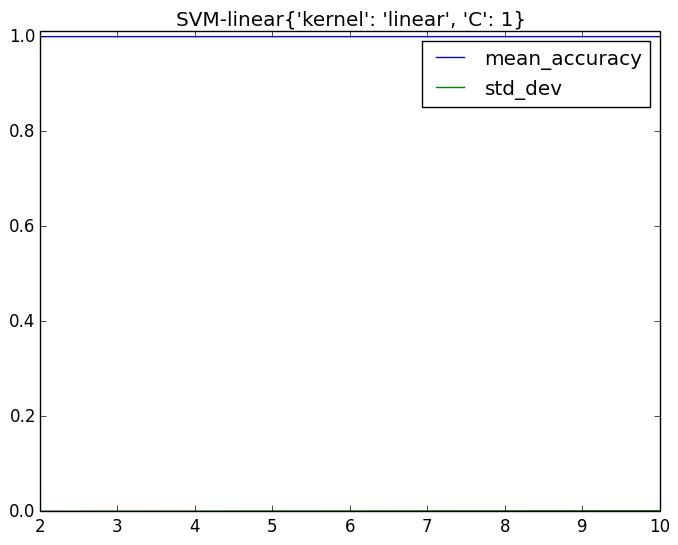
\includegraphics[scale=0.3]{model_accuracy_vs_folds_SVM-linear.png}
        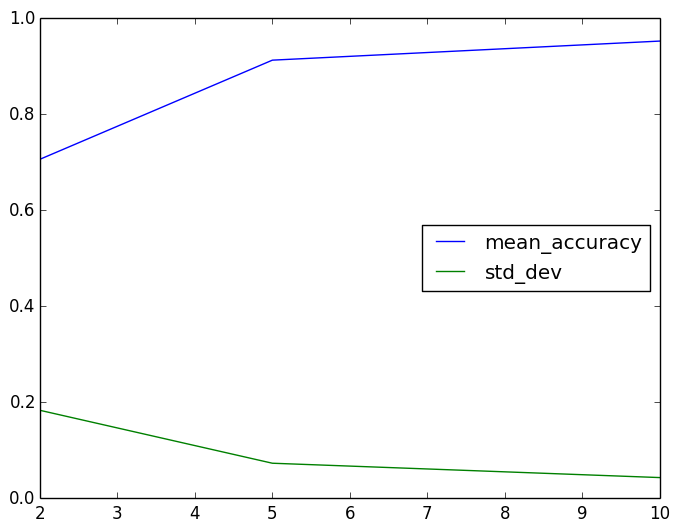
\includegraphics[scale=0.3]{model_accuracy_vs_folds_SVM-poly.png}
        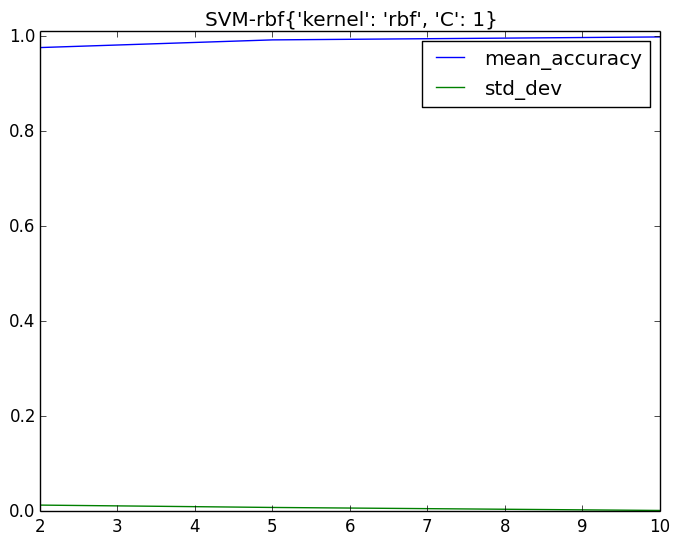
\includegraphics[scale=0.3]{model_accuracy_vs_folds_SVM-rbf.png}
    \end{center}
    \begin{center}
        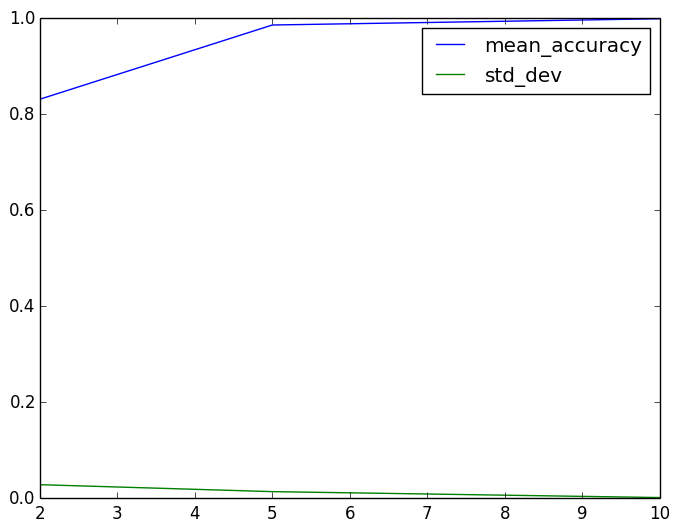
\includegraphics[scale=0.3]{model_accuracy_vs_folds_LR.png}
        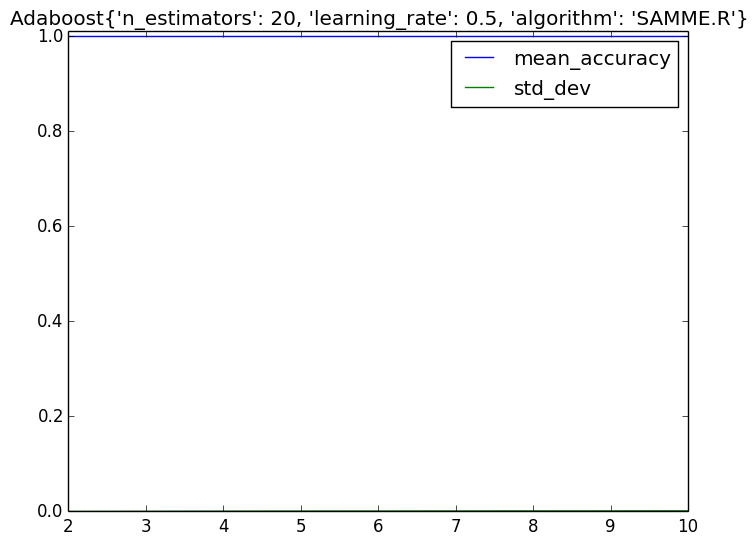
\includegraphics[scale=0.3]{model_accuracy_vs_folds_Adaboost.png}
    \end{center}

    The following table contains the mean and standard deviations of 5-fold CV for each of
    the models on this instance of running modelSelection.py.\\
    \begin{center}
        \begin{tabular}{llllll}
        Models   & Adaboost & Logistic Regression & SVM-Linear & SVM-RBF & SVM-Polynomial \\
        $\mu$    & 0.99937  & 0.99937             & 0.99906    & 0.99222 & 0.00840        \\
        $\sigma$ & 0.00076  & 0.00076             & 0.00076    & 0.96395 & 0.00711
        \end{tabular}
    \end{center}

    \subsection{ROC Curves}
    ROC is metric to evaluate classifier output quality. ROC is a plot of signal (True
    Positive Rate) against noise (False Positive Rate). The model performance is
    determined by looking at the area under the ROC curve (or AUC).\\

    ROC curves typically have the and false positive rate on the X axis and true positive
    rate on the Y axis. The top left corner of the plot is the “ideal” point - a false
    positive rate of zero, and a true positive rate of one. The “steepness” of ROC curves
    is also important, since it is ideal to maximize the true positive rate while
    minimizing the false positive rate. An ideal model would have AUC = 1.0, since it would
    mean that the false positive rate is zero for all observations. Here are the ROC
    Curves generated from the tuned hyperparameters for each model:

    \begin{center}
        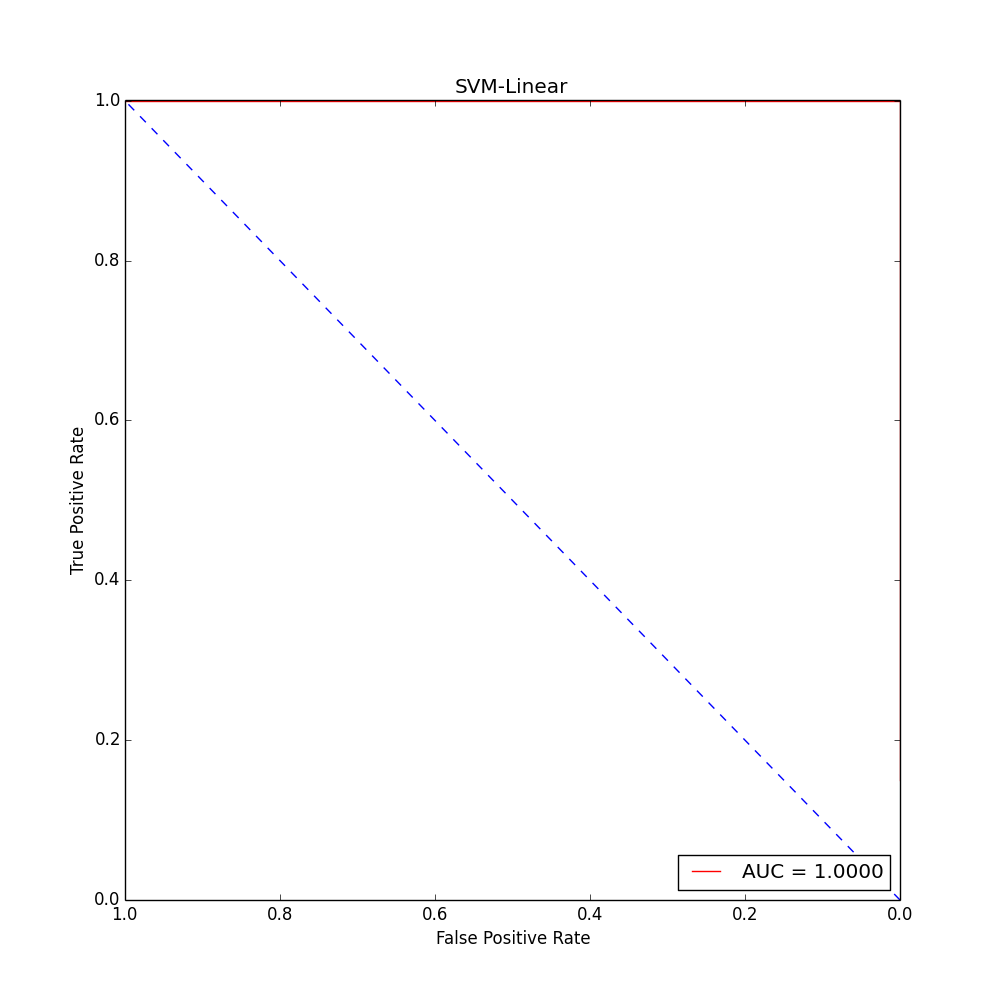
\includegraphics[scale=0.2]{roc_SVM-Linear.png}
        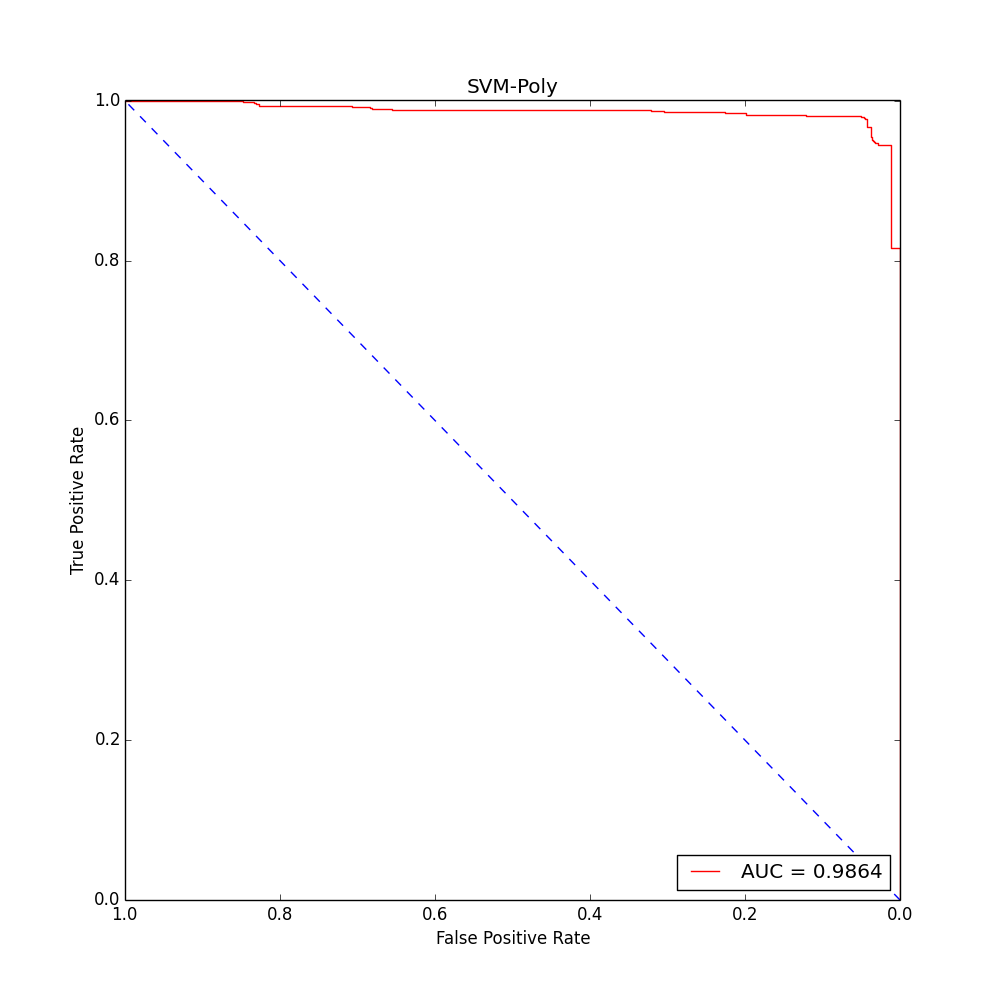
\includegraphics[scale=0.2]{roc_SVM-Poly.png}
        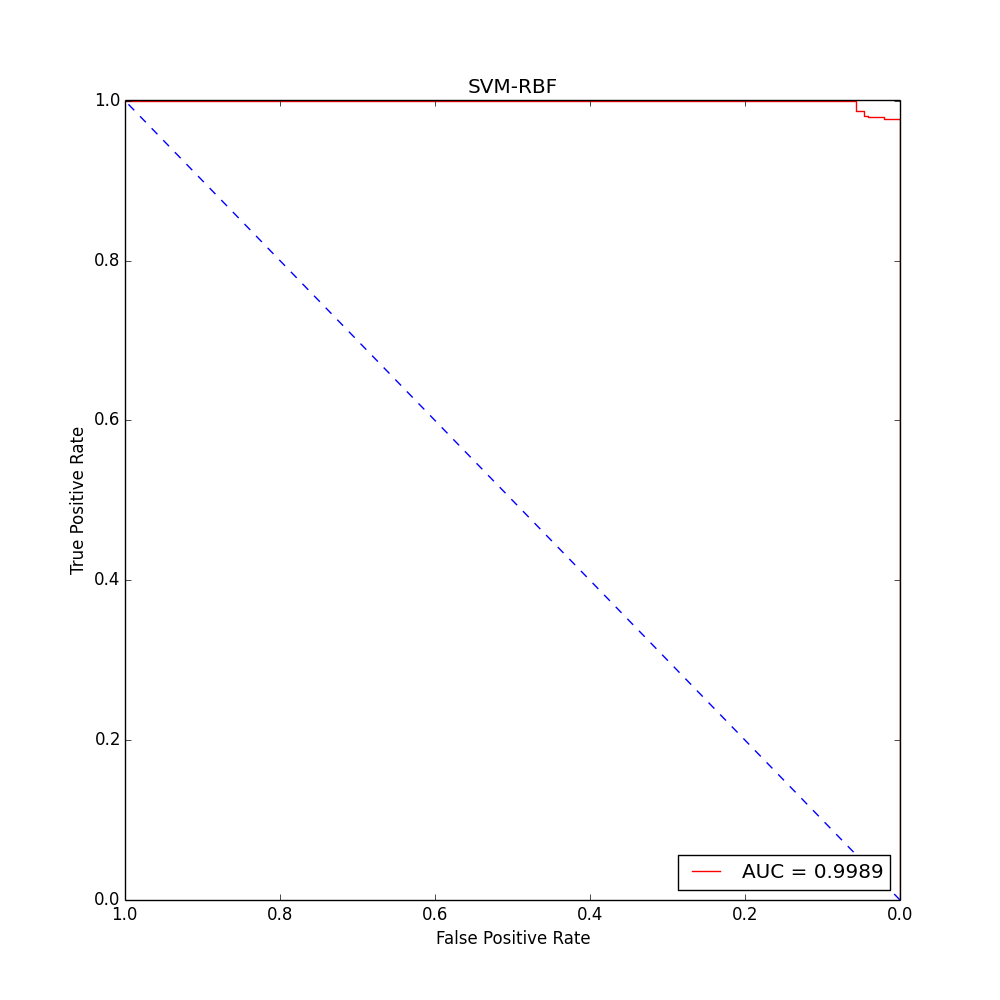
\includegraphics[scale=0.2]{roc_SVM-RBF.png}
    \end{center}
    \begin{center}
        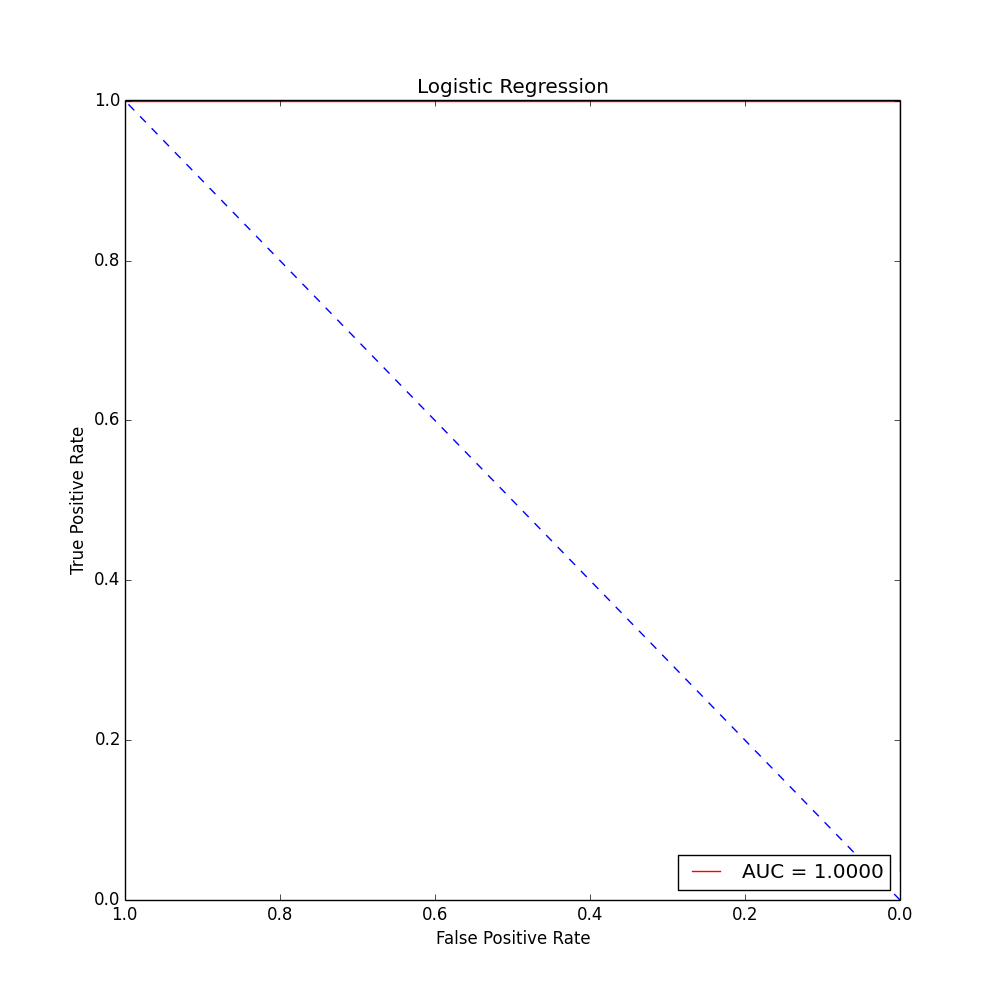
\includegraphics[scale=0.2]{roc_LR.png}
        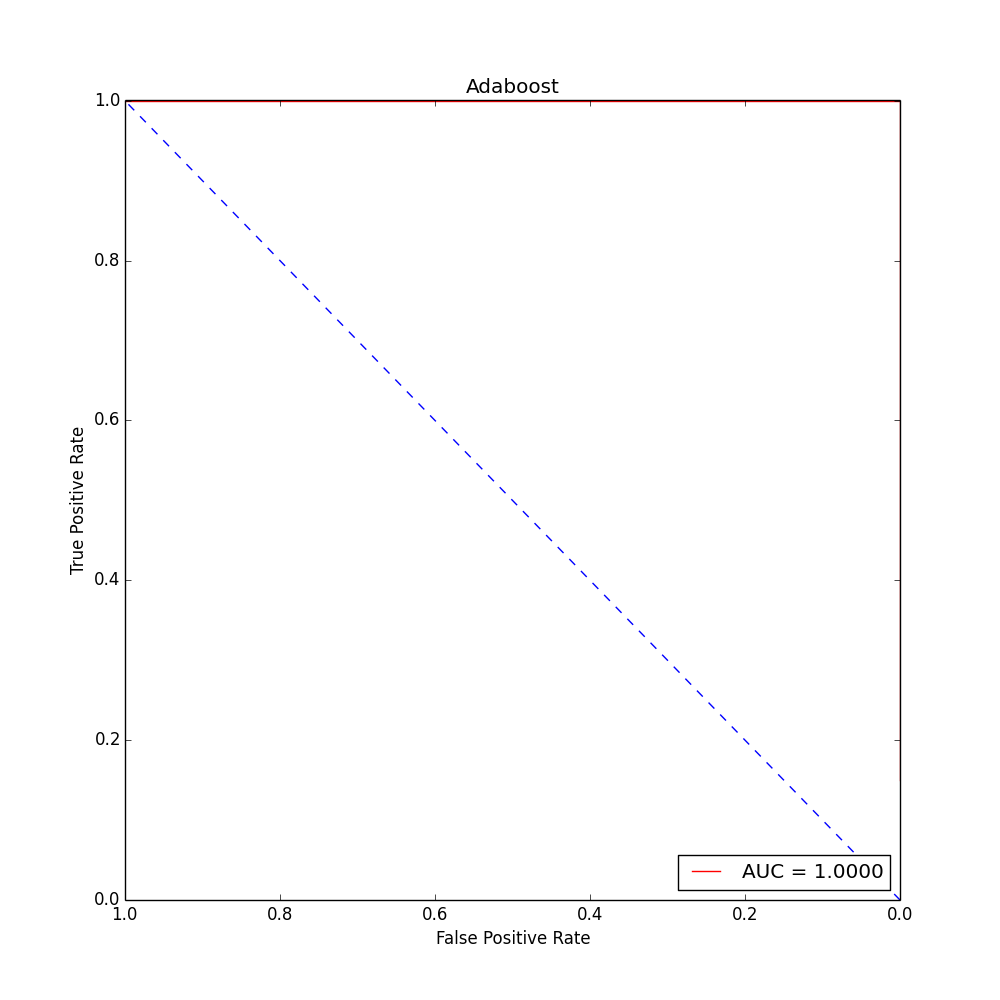
\includegraphics[scale=0.2]{roc_Adaboost.png}
    \end{center}


    \subsection{A Note Variability of Results}
    Recall that, as we mentioned in Section 4.2 and in Footnote 8, we are splitting the
    data into the three dataset we use for training and evaluation randomly. As such, the
    results obtained on different instances may be different. Furthermore, the tuned
    hyperparameters might be different as well.\\

    However, we obtain very good results when performing 2,5,10-fold cross-validation using the
    tuned SVM-linear, Logistic Regression, and Adaboost models consistently (more than 98\%
    accuracy  each time). As a result, we must employ other techniques such as statistical
    hypothesis testing and comparison of VC-Dimensions of these models to determine which
    model best fits our problem. We have done so in section 7. Regardless, we have presented
    the results for one such split of $ Z, Z'_1, Z'_2 $.

    % 7
    \section{Model Comparison}
    To compare the performance of different models based on the 5-fold cross validation on
    $ Z'_2 $, we can conduct hypothesis testing on their results. The purpose of hypothesis
    testing is to make a decision in the face of uncertainty. We used hypothesis testing
    to understand which model would be better to predict the edibility of the Mushrooms
    based on the data. Since none of our models are “perfect” we used hypothesis testing
    to understand which algorithm is more likely to perform better.

    \subsection{Hypothesis Testing}
    We used t-distribution because we don’t know the population standard deviation; we did
    not use all the mushroom data to train our algorithm. We ran $k$-fold cross validation
    for the different algorithms and compared them pairwise with t-distribution. We
    calculated the mean and standard deviation of the errors obtained from each of the
    $k$-folds. Let's call these mean errors $ \mu_1, \sigma_1 $ be the mean error and standard
    deviation of the first model and $ \mu_2, \sigma_2 $ be the mean error and standard
    deviation of the second model. We can conduct hypothesis testing as follows:
    \begin{enumerate}
        \item Null hypothesis: $ \mu_1= \mu_2 $
        \item Calculating test parameters:
            $$ x = \frac{(\mu_1-\mu_2)\sqrt{n}}{\sqrt{\sigma_1^2 + \sigma_2^2}} $$
        \item Calculating degrees of freedom:
            $$ \nu = \left\lceil \frac{(\sigma_1^2 + \sigma_2^2)^2 (n-1)}{\sigma_1^4 + \sigma_2^4} \right\rceil $$
        \item Reject null hypothesis in favor of first algorithm if
            $$ x > x_{1-\alpha, \nu} $$
            where $ \alpha $ is the level of significance (Note that we chose $ \alpha = 0.01 $).
    \end{enumerate}
    We conduct hypothesis test for the model with the best average performance against all
    the other models at the end of modelSelection.py using the t-test in hypothesisTest.py.
    The following are the results for one instance of running modelSelection.py (the same
    as the one for which results have been provided in section 6.1):
    \begin{lstlisting}
    Adaboost > LR: False
    Adaboost > SVM-linear: False
    Adaboost > SVM-rbf: False
    Adaboost > SVM-poly: True
    \end{lstlisting}
    As we can see on various instances, it is not clear even from hypothesis testing whether
    SVM-linear, Adaboost, or LogisticRegression are better suited to our problem. As a result,
    we must use some other way to compare how these models will

    \subsection{VC Dimensions and Generalizability}
    The Vapnik - Chervonenkis dimension of each model is given by:
        $$ d_{vc} = \max_n\{n: N_F(n)=2^n\} $$
    where $ N_F $ is the growth function.\\

    For our mushroom classification problem, we have tried multiple models and each of
    models display different characteristics for different train-test data splits and have
    differing accuracies and standard deviations. However, since each of them consistently
    have a performance of more than 98\% accuracy, and since hypothesis testing is
    inconclusive, we can use VC-dimensions for each of these models to get a theoretical
    upper bound on the test errors for each of the models. As such, the model with the best
    theoretical lower bound would be most suited to out problem.\\

    \begin{center}
        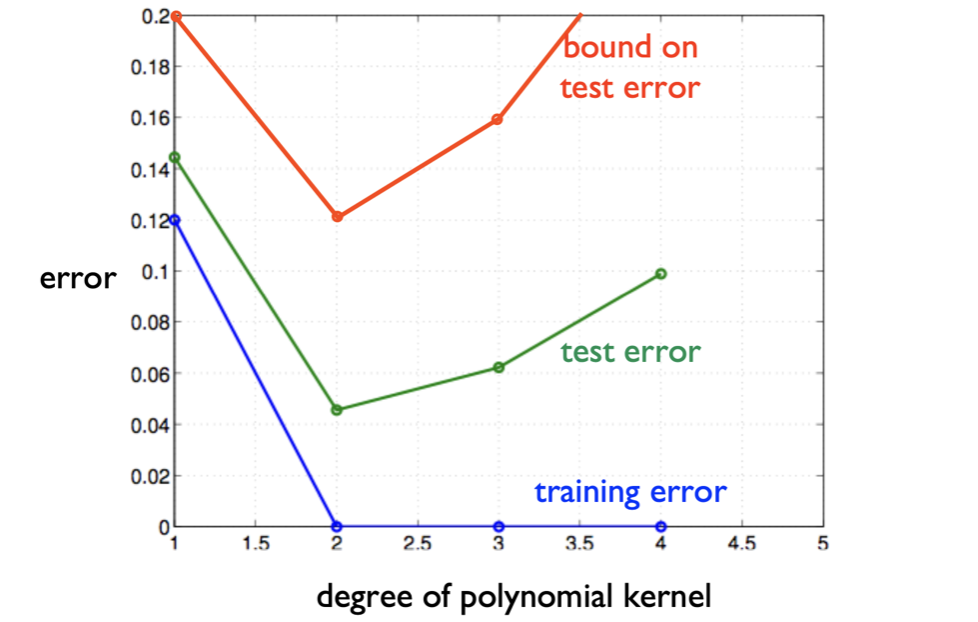
\includegraphics[scale=0.75]{vc.png}
    \end{center}

    The relation between the test error $ R(f) $, training error $ R_n(f) $ and VC-dimension
    is given by the following equation:
        $$ R(f) \leq R_n(f) + \sqrt{\frac{\log N_F(2n) + \log (4/\delta)}{n}} $$
    where it is true for $ N_F $ given that the number of samples $ n \geq d_{vc}$ (which, in
    our case it is) that:
        $$ \log N_F(2n) \leq d_{vc} \left(1+\log\frac{2n}{d_{vc}}\right) $$
    As a result, a model with lower vc-dimension would have an increased generalizability
    as it would result in a smaller upper bound for $ R_f $. The following are the
    VC-dimensions for all the models we use (where $ d $ = number of features,
    $ m $ = number of decision stumps):

    \begin{multicols}{2}
        \begin{enumerate}
            \item SVM Linear: $ d_{vc} = d + 1 $
            \item SVM RBF: $ d_{vc} = \infty $
            \item Logistic Regression: $ d_{vc} = d + 1 $
            \item Adaboost: $ d_{vc} \geq m/2 $
        \end{enumerate}
    \end{multicols}

    Since we are using $d=50$ features, we are using at most $20$ decision stumps for Adaboost,
    we know that Adaboost has a lower vc-Dimension than any of the other models we are using
    and would, as a result, have the lowest upper bound for the test error.

    % 8
    \section{Conclusion}
    After doing hypothesis testing we concluded that Adaboost, SVM linear and logistic
    regression perform equally well; when we compared each of them, we did not reject the
    null hypothesis (mean accuracy are equal). So, to choose the best out of these three
    we calculated the VC Dimension of each of these algorithms. As mentioned before,
    Adaboost has the lowest VC-Dimension out of these three models and thus has the lowest
    relative test-error bound. A lower test-error bound means that, theoretically, there
    is lesser gap between training error and testing error. Hence, with Adaboost we can be
    more certain about the testing error. Using feature selection in our algorithm
    discarded all the “noise” features and improved generalization. Exploring the data,
    helped us understand the correlations between the features and between a feature and
    the class label.

    % Appendices
    % Appendix A
    \newpage
    \section*{\underline{Appendix A: Data Description}}
    Classes: edible=e, poisonous=p (y-values)\\

    Size of dataset (before encoding): $ (n=8124, d=22) $

    Size of dataset (after encoding): $ (n=8124, d=107) $

    Attribute Information and Encoding:
    \begin{enumerate}
        \item \underline{Nominal Categorical Variables:}\\
        These variables will be encoded as binary one-hot features. As a result, each feature
        in this category would be replace by the $ k $ features in the encoded dataset if the
        feature has $ k $ possible values. These featues include:
        \begin{enumerate}[label=\roman*.]
            \item \textbf{cap-shape}:
                bell=b,
                conical=c,
                convex=x,
                flat=f,
                knobbed=k,
                sunken=s
            \item \textbf{cap-surface}:
                fibrous=f,
                grooves=g,
                scaly=y,
                smooth=s
            \item \textbf{cap-color}:
                brown=n,
                buff=b,
                cinnamon=c,
                gray=g,
                green=r,
                pink=p,
                purple=u,
                red=e,
                white=w,
                yellow=y
            \item \textbf{bruises}:
                bruises=t,
                no=f
            \item \textbf{odor}:
                almond=a,
                anise=l,
                creosote=c,
                fishy=y,
                foul=f,
                musty=m,
                none=n,
                pungent=p,
                spicy=s
            \item \textbf{gill-attachment}:
                attached=a,
                descending=d,
                free=f,
                notched=n
            \item \textbf{gill-color}:
                black=k,
                brown=n,
                buff=b,
                chocolate=h,
                gray=g,
                green=r,
                orange=o,
                pink=p,
                purple=u,
                red=e,
                white=w,
                yellow=y
            \item \textbf{stalk-root}:
                bulbous=b,
                club=c,
                cup=u,
                equal=e,
                rhizomorphs=z,
                rooted=r,
                missing=?
            \item \textbf{stalk-surface-above-ring}:
                fibrous=f,
                scaly=y,
                silky=k,
                smooth=s
            \item \textbf{stalk-surface-below-ring}:
                fibrous=f,
                scaly=y,
                silky=k,
                smooth=s
            \item \textbf{stalk-color-above-ring}:
                brown=n,
                buff=b,
                cinnamon=c,
                gray=g,
                orange=o,
                pink=p,
                red=e,
                white=w,
                yellow=y
            \item \textbf{stalk-color-below-ring}:
                brown=n,
                buff=b,
                cinnamon=c,
                gray=g,
                orange=o,
                pink=p,
                red=e,
                white=w,
                yellow=y
            \item \textbf{veil-type}:
                partial=p,
                universal=u
            \item \textbf{veil-color}:
                brown=n,
                orange=o,
                white=w,
                yellow=y
            \item \textbf{ring-type}:
                cobwebby=c,
                evanescent=e,
                flaring=f,
                large=l,
                none=n,
                pendant=p,
                sheathing=s,
                zone=z
            \item \textbf{spore-print-color}:
                black=k,
                brown=n,
                buff=b,
                chocolate=h,
                green=r,
                orange=o,
                purple=u,
                white=w,
                yellow=y
            \item \textbf{habitat}:
                grasses=g,
                leaves=l,
                meadows=m,
                paths=p,
                urban=u,
                waste=w,
                woods=d
        \end{enumerate}
        \item \underline{Ordinal Categorical Variables:}\\
        These variables will be encoded in place by encoding labels, as the data here has
        ordinal meaning to it. These variables include:
        \begin{enumerate}[label=\roman*.]
            \item \textbf{gill-spacing}:
                close=c$\to$0,
                crowded=w$\to$1,
                distant=d$\to$2
            \item \textbf{gill-size}:
                broad=b$\to$0,
                narrow=n$\to$1
            \item \textbf{stalk-shape}:
                enlarging=e$\to$0,
                tapering=t$\to$1
            \item \textbf{ring-number}:
                none=n$\to$0,
                one=o$\to$1,
                two=t$\to$2
            \item \textbf{population}:
                abundant=a$\to$0,
                clustered=c$\to$1,
                numerous=n$\to$2,
                scattered=s$\to$3,
                several=v$\to$4,
                solitary=y$\to$5
        \end{enumerate}
    \end{enumerate}

    % Appendix B
    \newpage
    \section*{\underline{Appendix B: List of Scripts}}
    The following scripts have been included with the preliminary report in the zip file:
    \begin{enumerate}
        \item data.py - Interface to load encoded data.
        \item project.py - Contains project config.
        \item kfoldcv.py - Conduct kfoldcv.
        % \item kfoldcv\_graph.py - Conduct kfoldcv for multiple models and multiple values
        % of $k$ and save the results.
        \item greedySubset.py - Conduct Greedy Subset Selection.
        \item featureSelection.py - Graph the results for Greedy Subset Selection.
        \item hyperparameterTuning.py - Tunes hyperparams for a model.
        \item hypothesisTest.py - Conducts hypothesis testing.
        \item rocCurve.py - Plots the ROC Curve for a model.
        \item models.py - Contains all models used and their hyperparameters.
        \item modelSelection.py - Main driver file. Makes calls to data, kfoldcv,
        hyperparameterTuning, hypothesisTest, models to conduct all discussed steps
        regarding model selection.
    \end{enumerate}


\end{document}
